%!TEX root = document.tex

%\subsection{Social Affinity Filtering}

Concatenating these ISAFs and ASAFs into 
feature vector $\x(u,i) = \langle
\cdots,X^{u,i}_{k},\cdots \rangle$ for 
$k \in \textit{Interaction-Classes} \cup \textit{Activity-Groups}$
(or any subset thereof), a SAF classifier is then simply a function
\begin{equation*}
f: \x(u,i) \to \likes(u,i),
\end{equation*}
where we restrict $\likes(u,i) \in \{ \true, \false \}$.\footnote{For
  training purposes, we omit any unobserved cases for which the class
  label $\likes(u,i)=\unknown$.  At prediction time, the binary
  classifier must always select a class label of $\true$ or $\false$.}  
Given a dataset of historical
observations $D = \{ \x(u,i) \to \likes(u,i) \}$, we can \emph{train} $f$
using any existing classification method; 
in this work we consider linear classifiers
trained by an SVM, logistic regression, or na\"{i}ve
Bayes.  For \emph{prediction}, given user $u$ and
item $i$, we build the feature vector $\x(u,i)$ and 
predict $\likes(u,i) = f(\x(u,i))$ using the trained
classifier $f$.\footnote{Since almost all classification
methods provide a score (or probability) of a classification, we
can also generate the top-$n$ item recommendations for a user $u$ by
sorting items by their score.}
%\footnote{In a \emph{recommendation} setting,
%one may not just want \emph{all} items $i$ that a user $u$ might
%like, rather one might want the top-$n$ items $i$ that a user $u$ is
%\emph{most likely} to like.  Fortunately, almost all classification
%methods provide a score or probability of a classification and hence
%items can be sorted by this score to extract the top-$n$.}

%%%%%%%%%%%%%%%%%%%%%%%%%%%%%%%%%%%%%%%%%%%%%%%%%%%%%%%%%%%%%%%%%%%%%%
%#suvash#
\begin{figure}[t!]
\centering
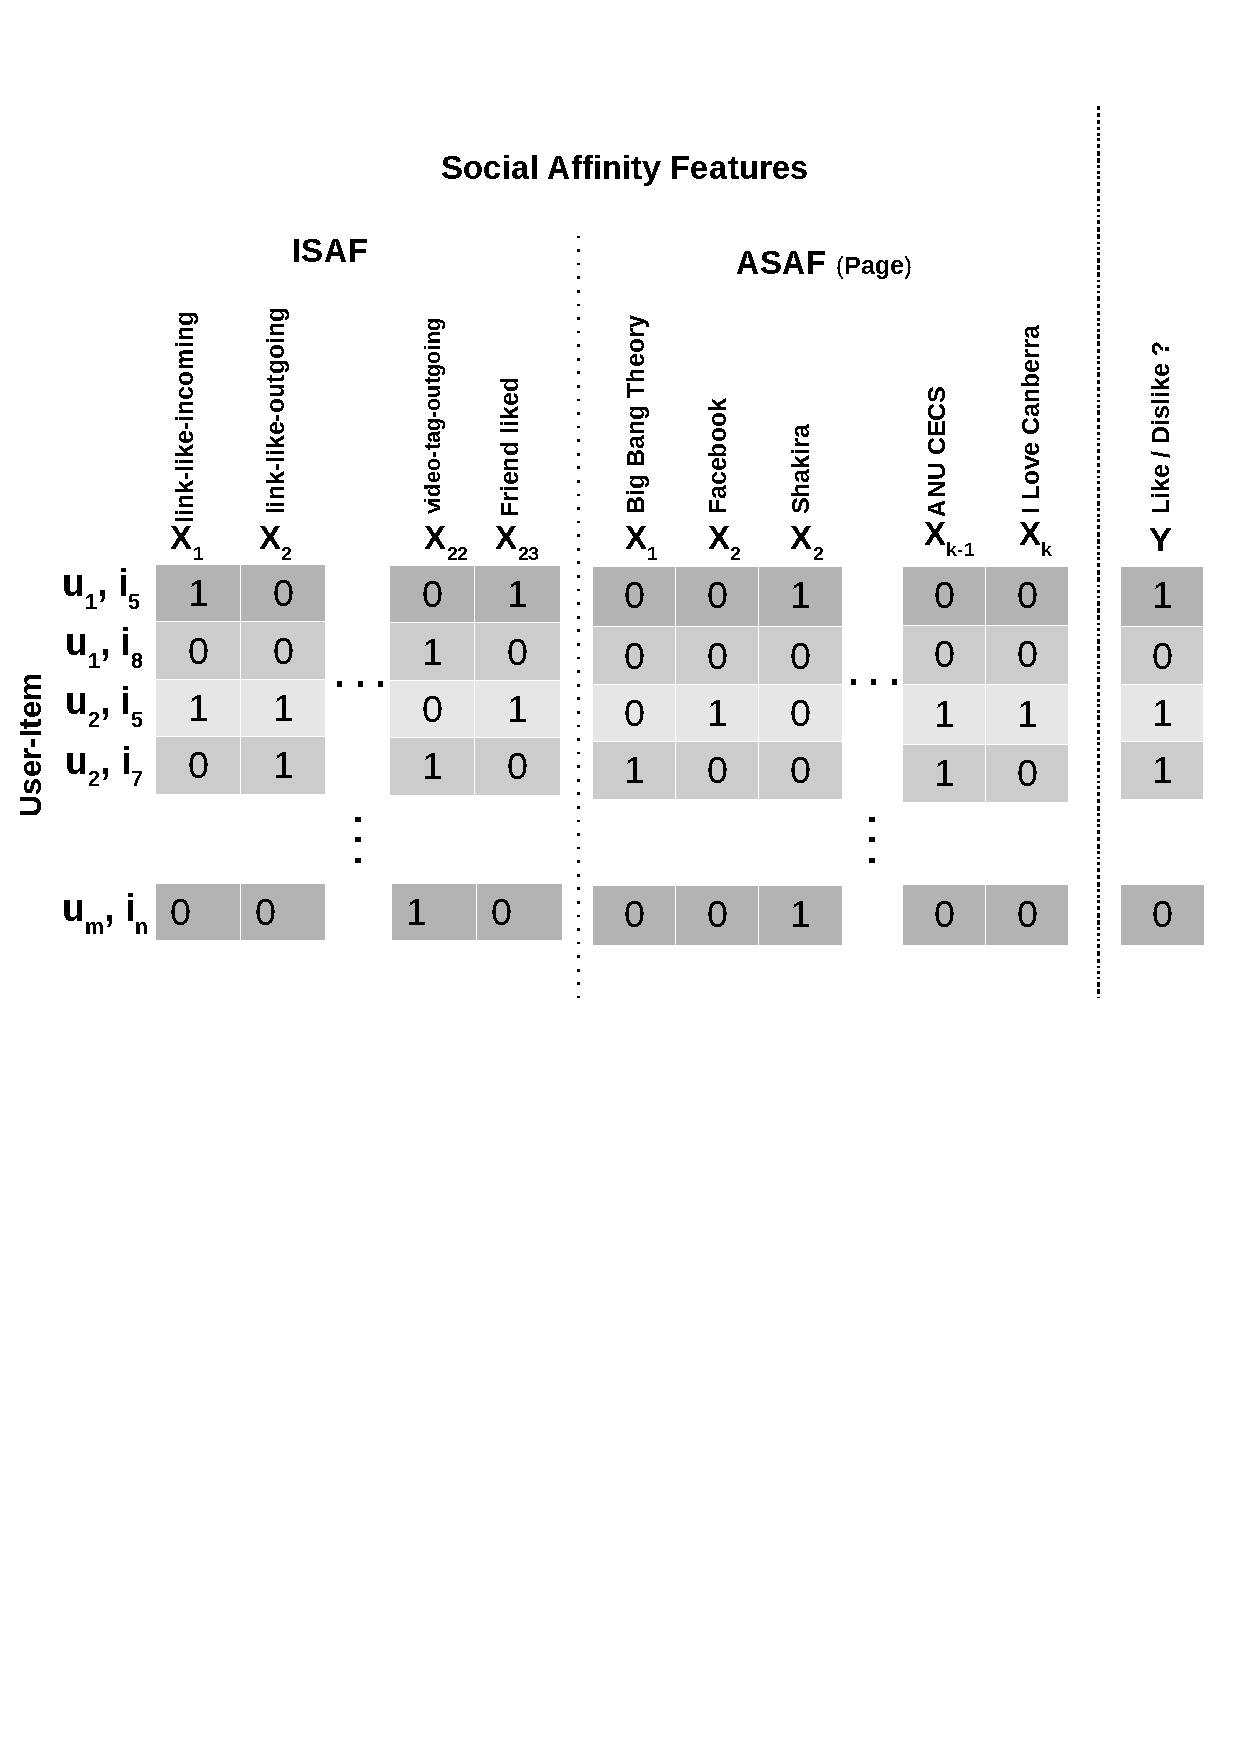
\includegraphics[width=1\linewidth]{data/plots/features/saf_features}
\caption{SAF training data example: each row corresponds to a training
  data sample for a specific user-item pair $(u,i)$ for which the
  prediction target $\like(u,i)$ is observed (last column).  All other
  columns represent the value of ISAF or ASAF features
  evaluated relative to the $(u,i)$ label of each row.
  All columns are binary-valued ($0=\false,1=\true$).}
\label{fig:features_overview}
\end{figure}
%#suvash#
%%%%%%%%%%%%%%%%%%%%%%%%%%%%%%%%%%%%%%%%%%%%%%%%%%%%%%%%%%%%%%%%%%%%%%

To understand how SAF works, it helps to visualise the training data as shown
in Fig~\ref{fig:features_overview}.  

\subsection{SAF vs. Other Filtering Methods}

While a classification approach to recommendation might evoke
comparisons to \emph{content-based filtering} (CBF)~\cite{newsweeder},
we remark that CBF is not a \emph{social} recommendation approach and
unlike CBF, SAF does not require explicit user features (e.g., age,
gender, location, etc.) or item descriptors (link text, link genre,
etc.); in contrast, SAF uses interaction and/or activity data for
social network users to define SAGs and learns the affinities between
a user (ego) and the different set of alters as defined by these SAGs.
Additionally, unlike state-of-the-art \emph{social collaborative filtering} 
approaches~\cite{socinf,rrmf,ste,sorec,sr,Noel2012NOF,lla}, SAF does
not aggregate user-user interaction and shared activity data into a
single aggregate statistic, instead it uses fine-grained distinctions
in this social data to define a large number of SAGs and learns which
of these SAGs are informative for recommendation.


